\documentclass[12pt]{article}

\usepackage[utf8]{inputenc}
\usepackage{url}
\usepackage{latexsym,amsfonts,amssymb,amsthm,amsmath}
\usepackage{mathtools}
\usepackage[sort&compress]{natbib}
\usepackage[french]{babel}
\usepackage[hidelinks,breaklinks=true]{hyperref}

%\usepackage[breaklinks=true]{hyperref} % For URLs
\usepackage{microtype}
\sloppy


\allowdisplaybreaks

\setlength{\parindent}{1em}
\setlength{\oddsidemargin}{0in}
\setlength{\textwidth}{6.5in}
\setlength{\textheight}{8.8in}
\setlength{\topmargin}{0in}
\setlength{\headheight}{18pt}

\usepackage[a4paper, margin=1.5in, bottom=2in]{geometry}
\setlength{\footskip}{15mm}

\title{Rapport Projet 2}
\author{Leader : Yannick Brenning \\ Followers : Kossi Kossivi, Nesrine Ghannay}

\begin{document}

\maketitle

\vspace{0.2in}

\section{Introduction} \label{introduction}

Ce projet étudie de quelques manières Word2Vec, un groupe de modèles pour la génération des plongements de mots statiques publié pour la première fois par \cite{DBLP:journals/corr/abs-1301-3781}. Dans ce document, deux architectures principales : CBOW (\textit{continuous bag-of-words}), et \textit{Skip-gram} ont été présentées. Dans ce cas, nous examinerons le modèle \textit{Skip-gram with negative sampling}, qui était introduit à la suite du document original par \cite{DBLP:conf/nips/MikolovSCCD13}. Les plongements générés par Word2Vec devraient être proches si les mots apparaissent dans les contextes similaires, comme ``bicyclette'' et ``vélo''.

Généralement, le modèle Skip-gram vise à prédire les mots qui apparaissent dans le contexte d'un certain mot cible. Nous entraînons un classifieur binaire sur les mots d'un corpus tel qu'il calcule la probabilité qu'un mot $c$ apparaît dans le contexte d'un mot cible $m$, écrit $P(+|m, c)$. De manière analogue pour les mots hors du contexte de $m$, nous notons $P(-|m, c)$. Ces probabilités sont calculées en utilisant la fonction sigmo\"\i de et le produit scalaire des vecteurs $\mathbf{m} $ et $ \mathbf{c} $ (voir les équations~\ref{eq:prob}), qui sont les plongements de $m$ et $c$. Les vecteurs sont stockés dans des matrices $\mathbf{M}$ et $\mathbf{C}$ telles que $\mathbf{M}$ contient les plongements pour chaque mot à la fin de l'apprentissage.

\begin{equation}\label{eq:prob}
\begin{split}
    P(+|m, c) & = \frac{1}{1 + \text{exp}(-\mathbf{m} \cdot \mathbf{c})} \\
    P(-|m, c) & = \frac{1}{1 + \text{exp}(\mathbf{m} \cdot \mathbf{c})} 
\end{split}
\end{equation}

Après la présentation du modèle initial dans la section suivante, nous explorerons quelques pistes concernant le sujet de ce projet.

La première piste est l'amélioration des performances. D'abord, nous comparons nos résultats avec le résultat de référence, mais il reste encore quelques possibilités d'amélioration. Notamment, \cite{DBLP:conf/nips/MikolovSCCD13} proposent une méthode d’échantillonnage des exemples négatifs, entre autres. En ce qui concerne le résultat de base, l'objectif d'atteindre des taux de réussite proches de ceux de la version originale de Word2Vec pourrait être intéressant.

Pour la deuxième piste, nous explorons les analogies, c'est-à-dire les associations d'idées entre les mots. Le principe de cette tâche est de faciliter les calculs simples avec les plongements de mots, par exemple \texttt{vector(roi) - vector(homme) + vector(femme)} $\;\approx\;$ \texttt{vector(reine)}. Cette propriété pourrait présenter un intérêt pour montrer que le modèle est capable d'encoder les relations linguistiques différentes.

\section{Modèle initial} \label{modèle initial}

Pour générer les plongements de mots avec un modèle de Word2Vec, nous avons d'abord besoin des données d'apprentissage. Dans le cadre de ce projet, nous utilisons ``Le Comte de Monte-Cristo'' comme corpus pour la création des données qui vont entraîner le modèle.

Nous commençons par tokeniser les mots du corpus, c'est-à-dire diviser le texte dans les \textit{tokens} afin de structurer et de simplifier le contenu pour le modèle. Sur la base de ces tokens, nous créons un vocabulaire avec lequel nous pouvons construire les exemples positifs et négatifs.

Pour la construction des exemples positifs, nous sélectionnons les mots qui apparaissent dans le contexte de chaque mot $m$ dans le vocabulaire. Le paramètre $L$ donne la taille du contexte, c'est-à-dire le nombre de mots précédant et suivant $m$ qui sont sélectionnés. Pour les exemples négatifs, l'approche na\"\i ve prend $k$ mots du lexique de façon aléatoire. 

\begin{equation}\label{eq:loss}
    L = -\lbrack \log \sigma(\mathbf{m} \cdot \mathbf{c}_{pos}) + \sum_{i=1}^k \log \sigma(-\mathbf{m} \cdot \mathbf{c}_{neg_i}) \rbrack
\end{equation}

En utilisant ces données et la descente du gradient de la fonction de perte donnée par l'équation~\ref{eq:loss}, nous réalisons le modèle de base. Un exemple positif et les $k$ exemples négatifs correspondants sont traités comme un \textit{minibatch}, sur lequel nous calculons le gradient pour la mise à jour des paramètres du modèle (équations~\ref{eq:update}). 

\begin{equation}\label{eq:update}
\begin{split}
    \mathbf{c}_{pos}^{t+1} & = \mathbf{c}_{pos}^t - \eta \lbrack \sigma(\mathbf{m} \cdot \mathbf{c}_{pos}^t) - 1 \rbrack \mathbf{m} \\
    \mathbf{c}_{neg}^{t+1} & = \mathbf{c}_{neg}^t - \eta \lbrack \sigma(\mathbf{m} \cdot \mathbf{c}_{neg}^t)\rbrack \mathbf{m} \\
    \mathbf{m}^{t+1} & = \mathbf{m}^t - \eta (\lbrack \sigma(\mathbf{m}^t \cdot \mathbf{c}_{pos}^t) - 1\rbrack \mathbf{c}_{pos}^t + \sum_{i=1}^k \lbrack \sigma(\mathbf{m}^t \cdot \mathbf{c}_{neg_i}^t) \rbrack \mathbf{c}_{neg_i}^t) \\
\end{split}
\end{equation}

Nous stockons la $\mathbf{M}$, qui contient les plongements de mots sous forme de vecteurs de colonne à l'issue de l'apprentissage, dans un fichier afin de l'évaluer sur un jeu d'évaluation. L'évaluation a lieu sur un ensemble de triplets de mots $(m, m_+, m_-)$ de sorte que le sens de $m_+$ soit plus proche de $m$ que $m_-$ de $m$. Pour chaque triplet, nous comparons les plongements des mots pour déterminer lequel est plus proche de $m$. En comptant le nombre de triplets qui passent le test $ \text{sim}(\mathbf{m}, \mathbf{m}_+) > \text{sim}(\mathbf{m}, \mathbf{m}_-)$, nous calculons le taux de réussite pour le modèle. Pour les comparaisons entre deux plongements de mot, nous utilisons la similarité cosinus comme mesure. 

Comme notre modèle suit les spécifications de \cite{DBLP:journals/corr/abs-1301-3781}, la fenêtre du contexte change sa taille aléatoirement entre $<1, L>$ pour chaque mot cible, ce qui accélère considérablement l'apprentissage. L'initialisation aléatoire des matrices suit d'ailleurs une distribution uniforme entre $[-\frac{0{,}5}{d}, \frac{0{,}5}{d})$, où $d$ est la dimension des plongements.

Le point de comparaison sur 10 expériences est un taux de réussite moyen de 53{,}2\% avec un écart type de 3{,}9 sur une configuration donnée de paramètres.\footnote{Dimension des plongements $d=100$, taille de fenêtre $L=2$, nombre d'exemples négatifs par exemple positif $k=10$, taux d'apprentissage $\eta=0{,}1$, nombre d'itérations $n\_ iter=5$, nombre minimum d'occurrences $minc=5$.} Lors de nos expériences, les résultats que nous avons obtenus avec notre implémentation de base sont un taux de réussite moyen de 63{,}8\% et un écart type de 2{,}2.

Concernant l'approche pour l'échantillonnage des exemples négatifs, nous pouvons constater quelques limitations potentielles. Tout d'abord, nous avons la possibilité de tirer un exemple positif par accident, car la sélection s'effectue sur l'ensemble du lexique. De plus, nous traitons tous les mots du vocabulaire de la même manière, ce qui n'est pas vraiment conforme à la réalité, où les fréquences et les niveaux d'informations contenues peuvent être très différents d'un mot à l'autre. Par exemple, les mots comme \texttt{le} ou \texttt{et} sont très fréquents, pourtant ils peuvent ne pas contenir autant d'informations que quelques mots plutôt rares. 

La même idée s'applique à la génération des exemples positifs, car la fenêtre contient souvent beaucoup de mots fréquents qui portent moins de signification que les mots moins fréquents. \cite{DBLP:conf/nips/MikolovSCCD13} mentionnent cela avec l'exemple du mot \texttt{France} : notre modèle Skip-gram bénéficie beaucoup plus de la cooccurrence avec \texttt{Paris} que la cooccurrence avec \texttt{la}. 

Les deux limitations mentionnées ci-dessus sont en rapport avec la première piste à creuser, dans laquelle nous essaierons d'améliorer les résultats du modèle précédemment détaillé.  

Une autre limitation est la taille du vocabulaire du corpus utilisé jusqu'à ce point. Pour s'attaquer au problème des analogies, nous utiliserons alors des plongements préexistants, entraînés sur le corpus plus large ``French CoNLL17'' par \cite{fares-etal-2017-word}. Pour comparer, le corpus utilisé jusqu'à ce point contient un vocabulaire de 3.210 mots, alors que celui utilisé par \cite{fares-etal-2017-word} contient 2.567.698 mots.

\section{Amélioration des performances} \label{amélioration des performances}

Afin d'améliorer le modèle Word2Vec, \cite{DBLP:conf/nips/MikolovSCCD13} proposent deux méthodes principales qui concernent le processus d'échantillonnage, appelées \textit{negative sampling} (échantillonnage négatif) et \textit{subsampling of frequent words} (sous-échantillonnage des mots fréquents). 

\subsection{Description} \label{description-1}

Premièrement, nous aborderons une différente méthode pour la sélection des exemples négatifs. Jusqu'à maintenant, nous choisissons les exemples négatifs aléatoirement d'une distribution uniforme sur l'ensemble des mots dans le lexique. 

\cite{DBLP:conf/nips/MikolovSCCD13} proposent une variation de la distribution d'unigramme en tant que distribution de probabilité pour le processus d'échantillonnage, parfois appelé distribution \textit{smooth} (lisse) d'unigramme \citep{levy2015improving}. Nous tirerons donc un exemple négatif $c_{neg}$ avec la probabilité $P(m)$ (voir l'équation~\ref{eq:unigram}), où $\#(m)$ désigne le nombre d'occurrences de $m$ dans le corpus. Le document original indique que les meilleurs résultats ont été obtenus en augmentant la distribution à une puissance de $\alpha = 0{,}75$, ce qui augmente les probabilités des mots rares. \cite{levy2015improving} démontrent ensuite les améliorations avec ce choix de paramètre, que nous utilisons aussi dans le cadre de l'expérience.

\begin{equation}\label{eq:unigram}
P(m) = \frac{\#(m)^{\alpha}}{\sum_{i=0}^n \#(m_i)^{\alpha}}
\end{equation}

L'effet de cette distribution est tel que la probabilité des mots rares augmente, et la probabilité des mots fréquents diminue (voir également la figure~\ref{fig:unigram}). PMI (Pointwise mutual information) est une mesure d'association entre les mots \citep{jurafsky2000speech}, tel que les grandes valeurs indiquent des associations fortes. \cite{levy2014neural} montrent que le modèle Skip-gram décrit par \cite{DBLP:conf/nips/MikolovSCCD13} calcule implicitement des plongements qui se rapprochent des valeurs PMI entre les mots et les contextes, moins une constante. Selon \cite{levy2015improving}, l'objectif du smoothing est alors de réduire le biais du PMI en faveur des mots rares. 

Avec ce changement, nous souhaitons donc améliorer la diversité des exemples négatifs sur lesquels nous entraînons le modèle afin d'améliorer le PMI et les performances.

La deuxième approche pour l'amélioration de Word2Vec est le sous-échantillonnage des exemples positifs. Dans les grands corpus, on observe aussi que les mots fréquents commencent à apparaître dans beaucoup de contextes. Cependant, l'information fournie par les mots comme \texttt{le}, \texttt{elle}, ou \texttt{un} n'est pas très utile. Dans l'autre sens, les plongements générés pour ces mots fréquents ne se changent pas beaucoup à partir d'un certain moment en raison du nombre considérable d'exemples d'entraînement. 

Pour compenser le déséquilibre des mots fréquents, \cite{DBLP:conf/nips/MikolovSCCD13} proposent d'éliminer un exemple positif avec la probabilité donnée par l'équation~\ref{eq:subsamp}, où $f(m)$ désigne la fréquence relative du mot $m$ dans le corpus, et $t$ est un paramètre \textit{threshold} (seuil), typiquement $10^{-5}$. Ce paramètre détermine le degré d'agressivité du sous-échantillonnage en ce qui concerne les mots avec des fréquences inférieures à $t$.

\begin{equation}\label{eq:subsamp}
P(m) = 1 - \sqrt{\frac{t}{f(m)}}
\end{equation}

En gardant à l'esprit ces approches, nous proposons les hypothèses suivantes :

\begin{enumerate}
    \item Le negative sampling améliorera les résultats des modèles de base de Word2Vec.
    \item En ajoutant le subsampling, on peut s'attendre à une amélioration des performances des modèles de base de Word2Vec.
    \item L'utilisation des deux méthodes ensemble devrait permettre une amélioration des performances des modèles de base de Word2Vec.
\end{enumerate}

\subsection{Mise en œuvre} \label{mise en œuvre-1}

Pour clarifier la mise en œuvre des améliorations, nous expliquerons d'abord brièvement la structure de l'implémentation. 

Notre modèle Word2Vec est structuré principalement en deux programmes ; la construction des données d'entraînement et le processus d'entraînement lui-même, ce qui diffère de la plupart des approches, où l'apprentissage et le traitement des données ont lieu en même temps. La structure utilisée dans cette expérience vise à améliorer la clarté et la simplicité de l'implémentation.

La mise en œuvre de la nouvelle méthode d'échantillonnage des exemples négatifs est assez simple. Après avoir construit les exemples positifs, nous créerons une distribution unigramme lisse sur le lexique en utilisant l'équation~\ref{eq:unigram}. À l'aide de la bibliothèque \texttt{numpy}, nous pouvons effectuer $k$ tirages sans remplacement selon cette distribution pour chaque exemple positif.

L'implémentation de l'échantillonnage des exemples positifs est un peu différente, car il existe différentes façons de procéder. D'abord, il est intéressant de noter que le code de Word2Vec utilise une formule différente pour l'implémentation de cette méthode, à savoir $ P(m) = \frac{f(m)-t}{f(m)} - \sqrt{\frac{t}{f(m)}} $, où $P(m)$ donne la probabilité de conserver le mot $m$ \citep{word2vec_source}. La raison pour cette différence n'est pas expliquée dans le document original, mais dans le cadre de cette expérience, nous notons des légères améliorations du temps d'exécution avec cette formule. De plus, l'implémentation originale utilise un seuil de $10^{-3}$ et non $10^{-5}$, ce que nous suivons pour cette mise en œuvre.

Par ailleurs, il y a des manières différentes concernant quand on effectue le sous-échantillonnage : soit on élimine les mots en ``glissant'' la fenêtre sur le corpus (c'est-à-dire on enlève les mots du contexte), soit nous éliminons les mots avant de glisser la fenêtre. Avec la deuxième option, que nous utiliserons dans cette expérience, nous aurons effectivement quelques mots dans les contextes qui n'auraient pas été présents avant le sous-échantillonnage. \cite{levy2015improving} ont appelé ce type de sous-échantillonnage ``dirty'' (sale) et ont constaté que les performances entre les deux options étaient comparables. Le processus de ce sous-échantillonnage aura donc lieu avant la construction des exemples d'entraînement ; nous parcourons le corpus et gardons chaque mot avec la probabilité $ P(m) = \frac{f(m)-t}{f(m)} - \sqrt{\frac{t}{f(m)}} $.

\subsection{Résultats} \label{résultats-1}

\begin{figure}[htpb]
    \centering
    \includegraphics[width=0.9\textwidth]{img/boxplot.png}
    \caption{Moyen taux de réussite sur 10 expériences avec les paramètres $d=100$, $L=2$, $k=10$, $\eta=0{,}1$, $n\_ iter=5$ et $minc=5$ pour chaque variation de modèle.}
    \label{fig:boxplot}
\end{figure}

La figure~\ref{fig:boxplot} montre les résultats de l'expérience. On voit que toutes les variations du modèle de base montrent des améliorations à différents degrés. Bien que les taux moyens s'améliorent, les variabilités entre les résultats de chaque modèle augmentent également. 

Le modèle de base donne des résultats relativement cohérents vers 63\%, ce qui est déjà une amélioration de notre point de comparaison. Le negative sampling entraîne de légères améliorations, avec un taux de réussite moyen de 66{,}8\% et un écart type de 2{,}8\%. Pour cette expérience, nous pouvons alors confirmer notre première hypothèse. 

Notamment, les taux de réussite moyens du modèle avec subsampling et du modèle avec les deux méthodes ensemble dépassent les 70\% avec respectivement 70{,}2\% (écart type de 3{,}9\%) et 73{,}7\% (écart type de 4{,}3).

Malgré de meilleurs résultats pour les taux de réussite moyens, les écarts types sont assez larges, ce qui peut indiquer des résultats légèrement incohérents. Toutefois, cela peut également résulter de la configuration de notre expérience, puisque nous n'avons suivi que 10 passages pour calculer les scores moyens. 

Afin de mieux examiner ces résultats et de les améliorer, il serait possible de comparer les variations en fonction des différentes méthodes d'initialisation et des modifications du type de fenêtre. En plus, on pourrait expérimenter avec des options de tokenisation plus optimales, ainsi que l'augmentation du nombre d'expériences, ce qui n’entre pas dans le cadre de ce travail.

\section{Analogies} \label{analogies}

Comme mentionné précédemment, les plongements de mots permettent également de faire des calculs simples, comme \texttt{vector(roi) - vector(homme) + vector(femme)} $\;\approx\;$ \texttt{vector(reine)}. Pour examiner cette capacité, nous suivons la tâche posée par \cite{DBLP:journals/corr/abs-1301-3781} avec des plongements préexistants de \cite{fares-etal-2017-word}. Un parti des plongements utilisé à cette fin est visualisé par la figure~\ref{fig:embeddings}. 

\subsection{Description} \label{description-2}

Pour examiner le raisonnement analogique des plongements de mots, nous devons utiliser les distances entre les vecteurs pour déterminer quel plongement est le plus proche du résultat de notre calcul. Pour un ensemble de plongements $V = \{e_1, \dotsc, e_N\}$ et un plongement particulier $x \notin V$, nous cherchons trouver l'élément de $ V $ la plus proche de $x$ (voir l'équation~\ref{eq:dist}).\footnote{Pour cette expérience, la mesure de la distance $d$ est toujours euclidienne.}

\begin{equation}\label{eq:dist}
    \hat{e} = \underset{e \in V}{\text{argmin }} d(e, x)
\end{equation}

Comme indiqué en section~\ref{modèle initial}, la taille du vocabulaire est très grande, ce qui rend les recherches naïves coûteuses. Afin de trouver les solutions plus efficacement, nous utilisons donc un arbre $k$-$d$, qui permet des recherches plus rapides dans les espaces à $k$ dimensions. \citep{bentley1975multidimensional}. 

Notre hypothèse pour la présente section est alors que l'utilisation des arbres $k$-$d$ permettra des calculs d'analogies plus rapides que le parcours na\"\i f de l'espace.

\subsection{Mise en œuvre} \label{mise en œuvre-2}

Car les plongements existent déjà, la mise en œuvre se compose de trois parties principales : la lecture des plongements donnés, l'implémentation de l'arbre $k$-$d$, et la construction d'un jeu de données pour l'évaluation.

D'abord, la lecture des plongements a posé une difficulté à cause de la taille immense. Étant donné que ce projet est réalisé avec une infrastructure de calcul limitée, effectuer des opérations sur des données occupant $\approx 2{,}5$ GB d'espace en mémoire n'est pas possible. Vu que les plongements sont triés dans l'ordre décroissant de fréquence, nous utilisons d'abord les premières 500.000 plongements pour nos calculs.

Nous avons d'abord implémenté la structure d'un arbre $k$-$d$ ainsi que l'algorithme de recherche selon la définition de \cite{friedman1977algorithm}, en utilisant une classe \texttt{KDTree} composée récursivement de nœuds \texttt{Node}.

Cette implémentation a entraîné des difficultés en ce qui concerne la mémoire vive disponible, car la construction implémentée dans ce cas nécessite $2 \cdot |V|$ stockés en mémoire.\footnote{La construction de l'arbre $k$-$d$ s'effectue à partir de la liste de plongements, ce qui signifie qu'à la fin de la construction, nous avons au moins $2 \cdot |V|$ éléments stockés en mémoire.} Pour le cadre de cette expérience, nous utilisons alors 100.000 plongements. Nous comparerons les durées d'exécution des recherches avec les arbres $k$-$d$ à celles des recherches exhaustives (c'est-à-dire des parcours na\"\i fs de l'espace).

% La bibliothèque Scikit-Learn \citep{scikit-learn} contient un implémentation des arbres $k$-$d$ que nous avons utilisé afin de comparer les résultats, ainsi que la recherche exhaustive (c'est-à-dire le parcours na\"\i ve de l'espace).
% Les données ont posé d'autres problèmes, notamment lorsqu'il s'agissait de la construction des arbres $k$-$d$. 

Pour l'évaluation, nous créerons un ensemble de 100 analogies différentes en suivant le format \texttt{(homme, roi, femme, reine)}, ce qui signifie un calcul \texttt{vector(roi) - vector(homme) + vector(femme)} $\approx$ \texttt{vector(reine)}. Nous enregistrerons la durée d'exécution de la recherche du plus proche voisin pour le vecteur obtenu. Ensuite, nous comparerons le voisin trouvé avec le quatrième mot de la ligne, en comptant le nombre total des résultats ``corrects''.\footnote{Bien entendu, ce nombre restera toujours le même, car les plongements et les analogies sont statiques.}

\subsection{Résultats} \label{résultats-2}

\begin{figure}[htpb]
    \centering
    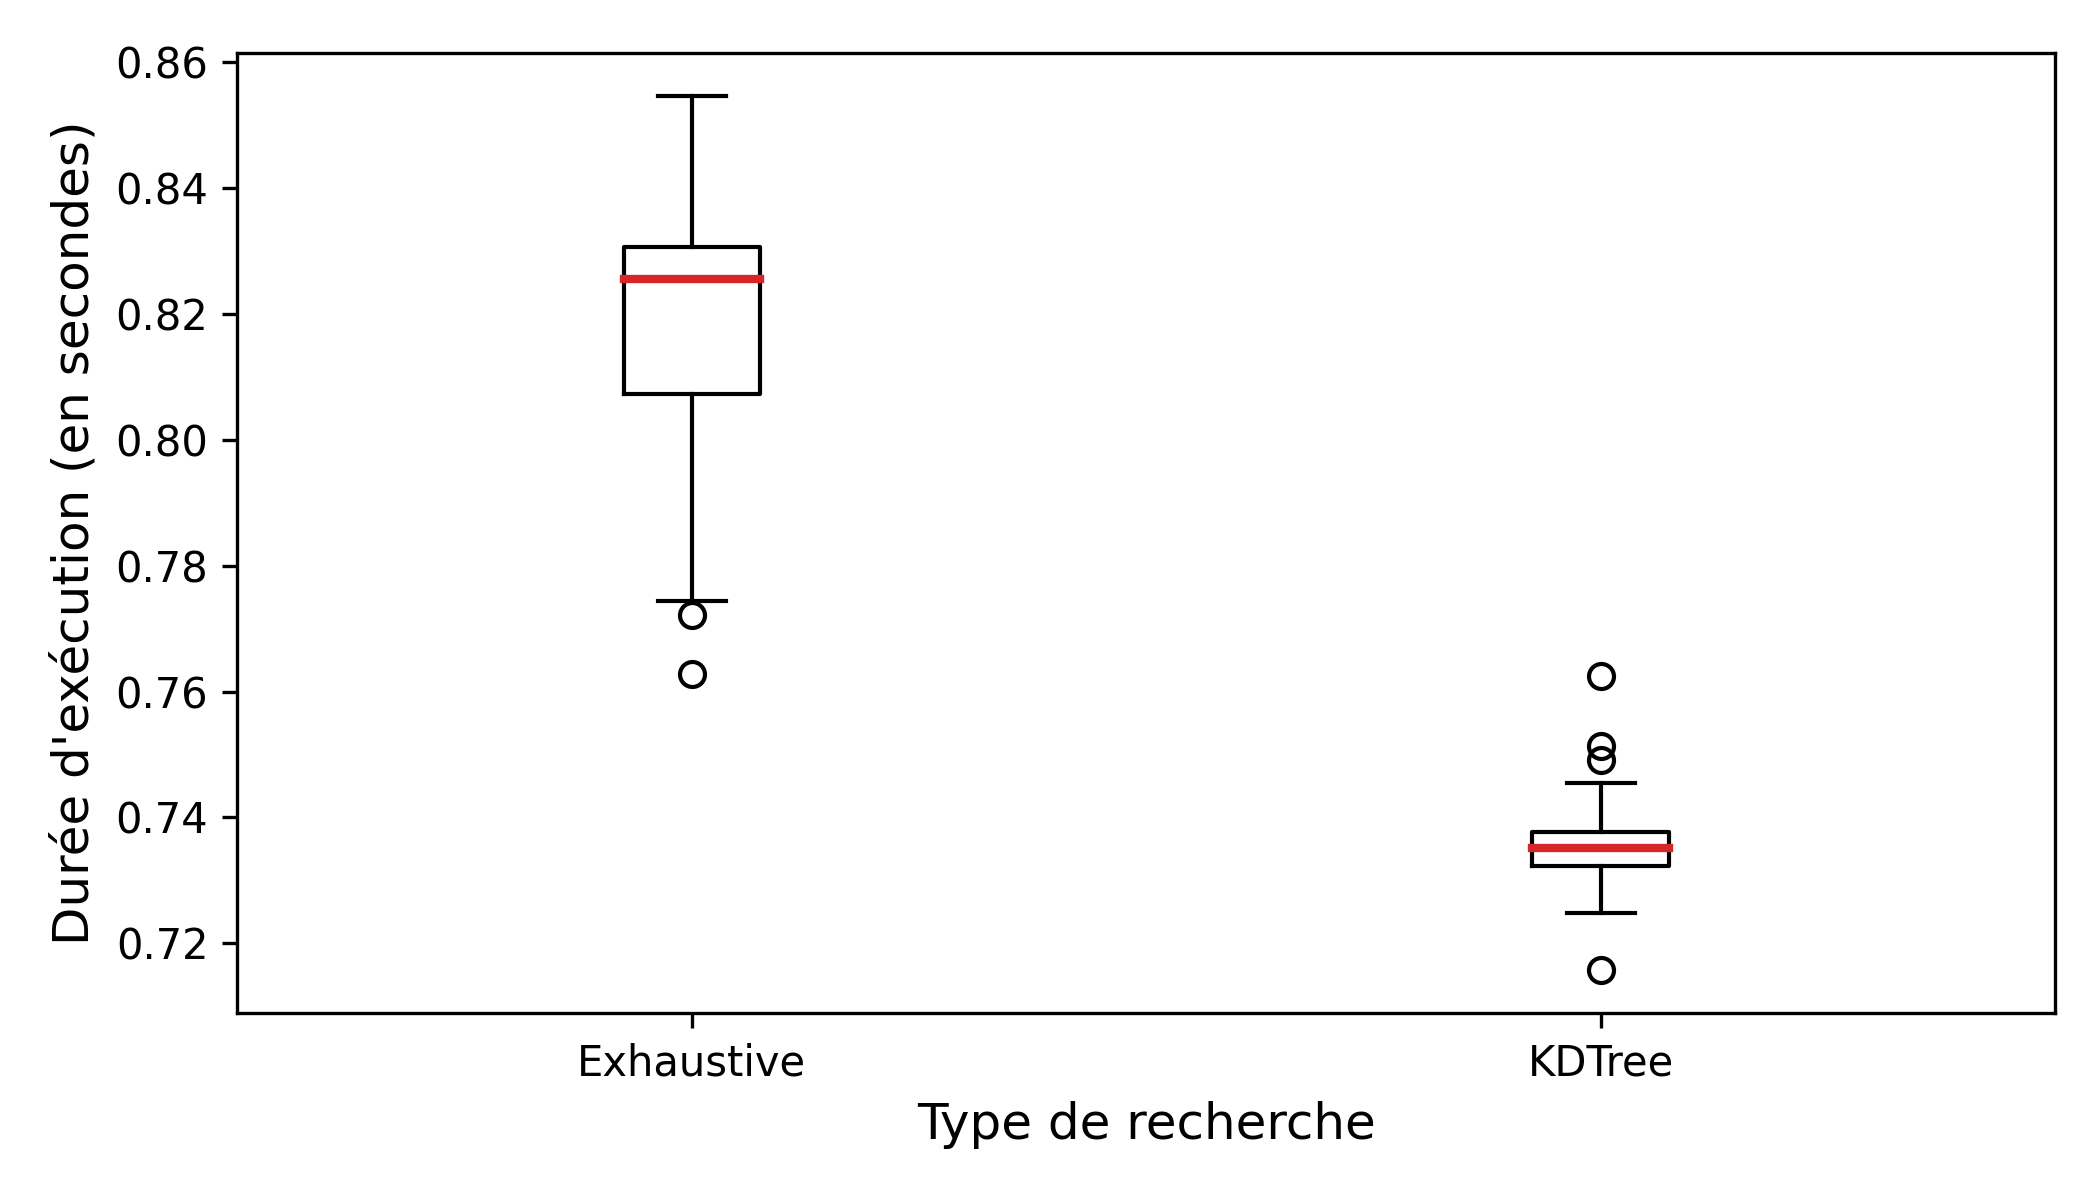
\includegraphics[width=0.8\textwidth]{img/times.png}
    \caption{Durée d'exécution en secondes pour chaque recherche du plus proche voisin du vecteur calculé par \texttt{vector(A) + vector(B) - vector(C)}.}
    \label{fig:times}
\end{figure}

Pour chaque façon de recherche, nous avons suivi les durées d'exécution pour les calculs des analogies (c'est-à-dire la recherche du plus proche voisin dans l'espace des plongements). Nous montrons les résultats dans la figure~\ref{fig:times}. Bien entendu, ces scores dépendent fortement de la machine et ne sont donc pas nécessairement représentatifs, mais ils serviront de points de référence généraux dans le contexte de cette expérience. 

L'approche na\"\i ve prend un moyen de 0{,}819 secondes pour chaque recherche, avec un écart type de 0{,}019, tandis que l'implémentation de l'arbre $k$-$d$ effectue les recherches avec une durée moyenne de 0{,}735 secondes et un écart type de 0{,}006. La figure~\ref{fig:times} indique aussi des résultats plus cohérents avec l'arbre $k$-$d$. Le résultat de l'évaluation sur les 100 analogies est un taux de réussite de 49\%. Il est important de souligner que ce résultat peut dépendre fortement des analogies utilisées.

En rapport avec notre hypothèse, nous pouvons donc affirmer que les calculs sont légèrement plus rapides, mais seulement par une faible marge, et en limitant le nombre de plongements utilisés. Globalement, nous pouvons dire que l'application de cette implémentation de l'arbre $k$-$d$ n'est pas nécessairement utile dans cette tâche spécifique.

Une raison pour ces résultats pourrait être un phénomène appelé \textit{curse of dimensionality} (le fléau de la dimension) par \cite{Freimer1961AdaptiveCP}, qui s'applique notamment aux tâches de recherche des plus proches voisins. Comme règle générale, on constate que pour des données en dimension $ k $, le nombre de points $ n $ devrait être $ n \gg 2^k $ pour que cette recherche soit efficace \citep{indyk2004nearest}. Si ce n'est pas le cas, cette méthode pourrait ne pas être beaucoup plus rapide qu'une recherche exhaustive.

En plus, l'implémentation de l'arbre $k$-$d$ utilisé ici est assez simple, alors que les implémentations utilisées dans les bibliothèques comme Scikit-Learn utilisent des méthodes plus sophistiquées comme le pruning et les fonctionnalités de Cython \citep{behnel2011cython} ; une telle mise en œuvre surpasse le cadre de ce rapport. 
\newpage
\section{Conclusions et perspectives} \label{conclusions et perspectives}

Le but de ce rapport était d'examiner le modèle Word2Vec et ses capacités dans quelques aspects. Surtout, nous avons exploré l'effet des méthodes d'améliorations présentées par \cite{DBLP:conf/nips/MikolovSCCD13} ainsi que l'aspect de l'évaluation des analogies.

En ce qui concerne ses sujets, nous avons posé trois hypothèses sur les méthodes d'amélioration et une hypothèse sur l'évaluation des analogies. Nous avons créé, exécuté et évalué deux expériences afin de répondre aux hypothèses. Les trois hypothèses sur le premier sujet ont été confirmées en montrant les améliorations sur le modèle de base, tandis que l'hypothèse du deuxième sujet avait des résultats mitigés. Les expériences ont montré plusieurs aspects intéressants du modèle Word2Vec, notamment les influences des différentes méthodes d'échantillonnage sur les performances du modèle et la capacité de l'inférence des analogies. 

Il existe pourtant des possibilités d'élargir le cadre des expériences en quelques aspects. Comme mentionné précédemment, une meilleure infrastructure de calcul pourrait faciliter les recherches sur plus de plongements et la construction des arbres $k$-$d$ plus grandes. Par contre, l'utilisation d'une approche approximative qui est plus efficace sur les données de larges dimensions comme le ``Locality Sensitive Hashing'' pourrait aussi conduire à de meilleurs résultats \citep{andoni2008near}. D'ailleurs, les aspects qui concernent l'entraînement du modèle, comme la taille de la fenêtre ou l'effet d'une fenêtre dynamique par rapport à une fenêtre non dynamique, n'ont pas été explorés. En examinant ces aspects, entre autres, on pourrait mieux comprendre et aborder les sujets présentés dans ce rapport. 

\newpage

\bibliographystyle{plainnat}
\bibliography{literature} 

\appendix
\section{Figures supplémentaires}

\begin{figure}[htpb]
    \centering
    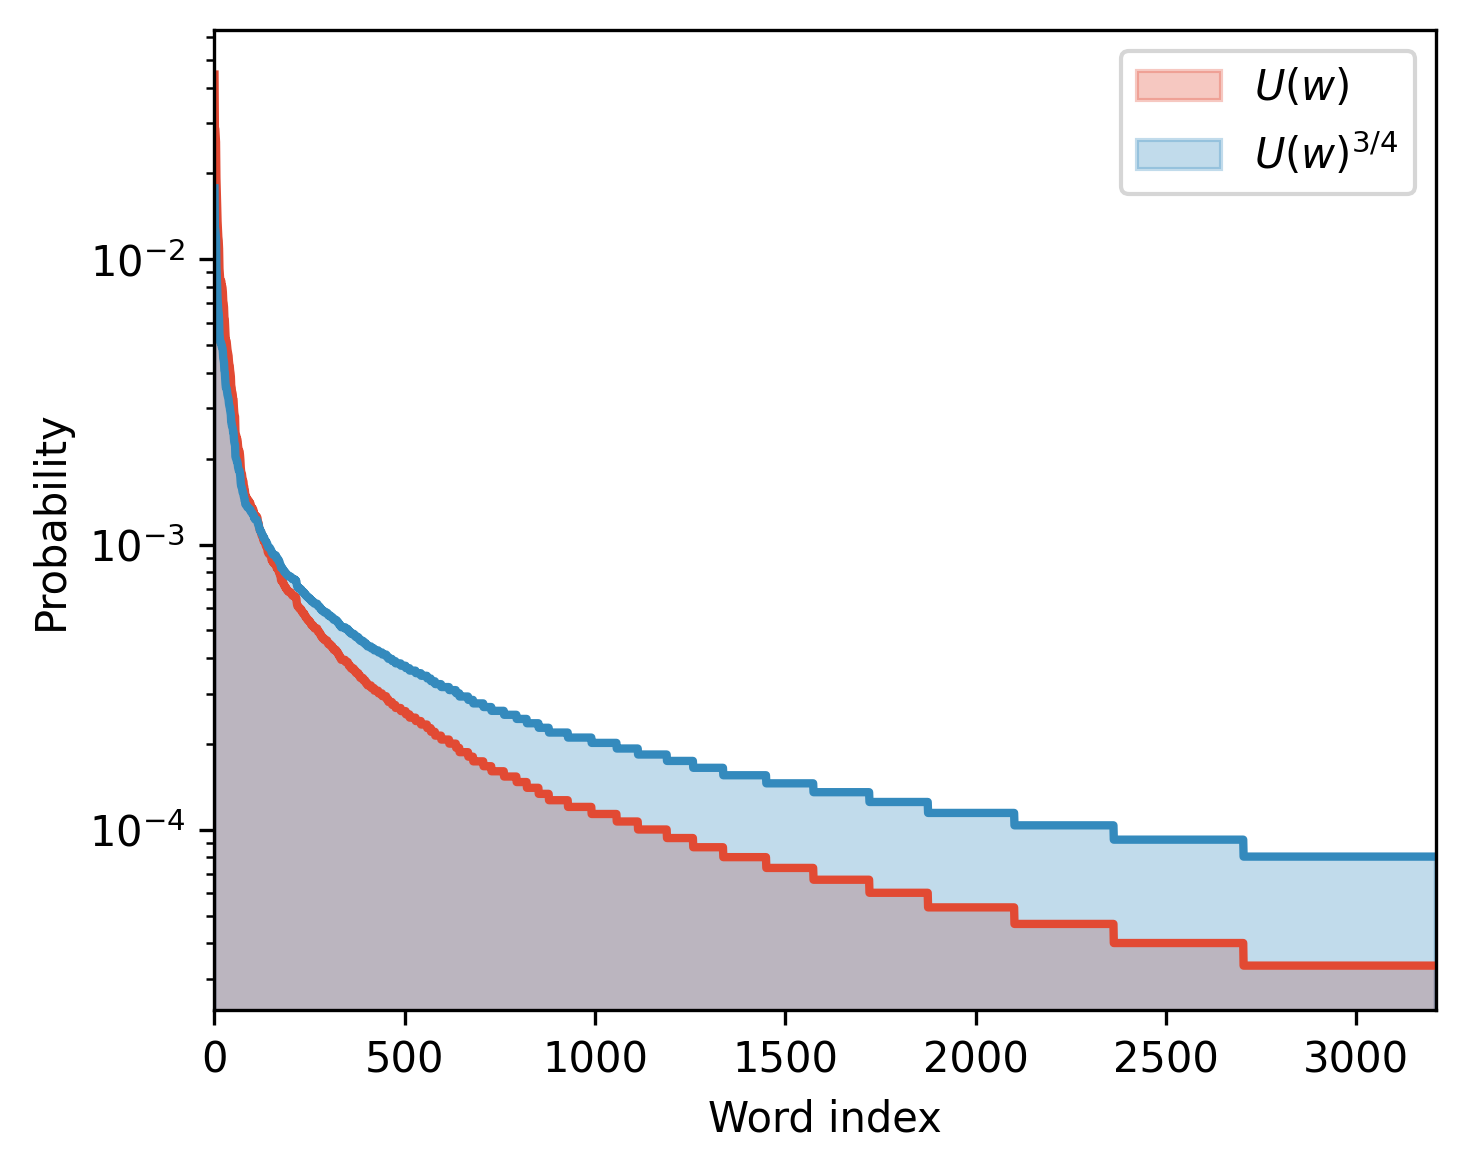
\includegraphics[width=0.6\textwidth]{img/unigram.png}
    \caption{Probabilité de tirer chaque mot du lexique selon la distribution unigramme (rouge) et la distribution unigramme à la puissance 0{,}75 (bleu) avec $minc = 5$.}
    \label{fig:unigram}
\end{figure}

\newpage
\clearpage
\vspace*{-1in}
\begin{figure}[t!]
    \centering
    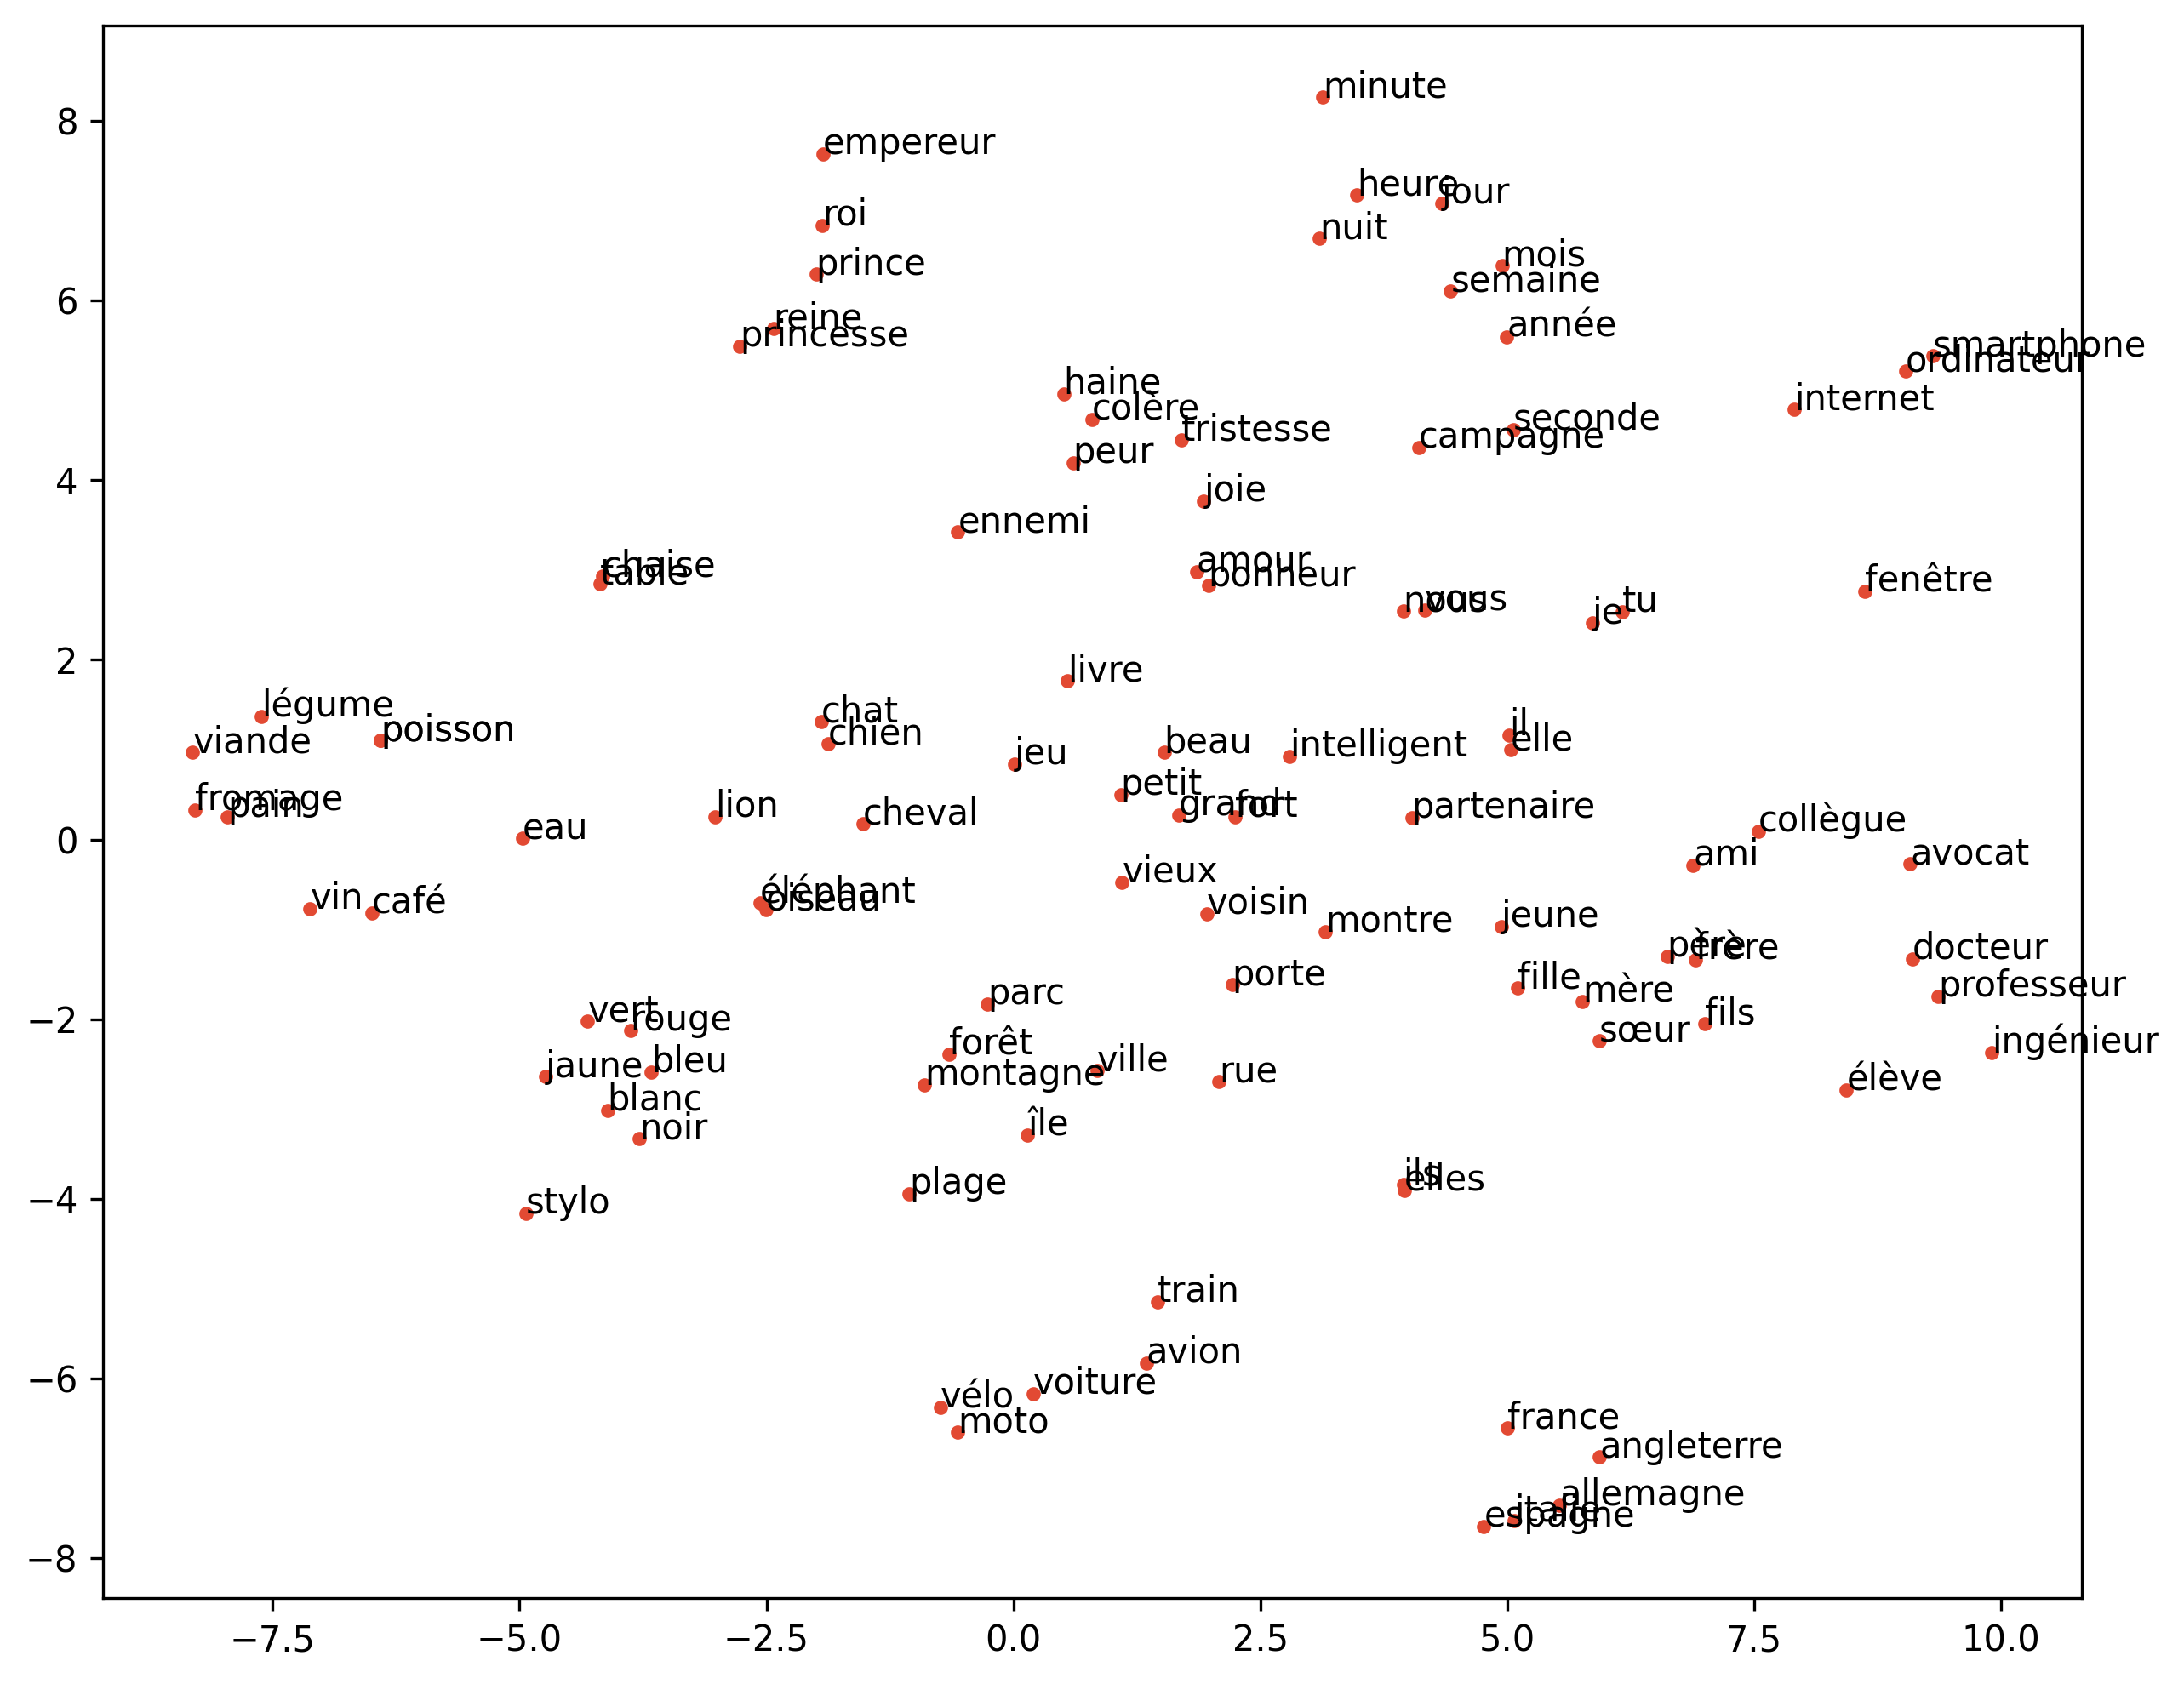
\includegraphics[width=0.9\textwidth]{img/embedding_plot.png}
    \caption{Visualisation des plongements réduits de 100 mots différents de \cite{fares-etal-2017-word}. La réduction de 100 à deux dimensions a lieu avec t-SNE \citep{van2008visualizing}.}
    \label{fig:embeddings}
\end{figure}

\end{document}
